\documentclass[twoside,11pt]{article}
\usepackage{jmlr2e}
\usepackage{graphicx}
\graphicspath{ {./images/} }
\usepackage{enumitem}
\newlist{mylistenv}{enumerate}{3}
\newenvironment{mylist}[1]{%
	\setlist[mylistenv]{label=#1\arabic{mylistenvi}.,ref=#1\arabic{mylistenvi}}%
	\setlist[mylistenv,2]{label=#1\arabic{mylistenvi}.\arabic{mylistenvii}.,ref=#1\arabic{mylistenvi}.\arabic{mylistenvii}}%
	\setlist[mylistenv,3]{label=#1\arabic{mylistenvi}.\arabic{mylistenvii}.\arabic{mylistenviii}.,ref=#1\arabic{mylistenvi}.\arabic{mylistenvii}.\arabic{mylistenviii}}%
	\renewenvironment{mylist}{\begin{mylistenv}}{\end{mylistenv}}
	\begin{mylistenv}%
	}{%
	\end{mylistenv}%
}
\newcommand\tab[1][1cm]{\hspace*{#1}}

% Definitions of handy macros can go here

\newcommand{\dataset}{{\cal D}}
\newcommand{\fracpartial}[2]{\frac{\partial #1}{\partial  #2}}


\firstpageno{1}

\begin{document}

\title{Project 3: Decision Trees for Classification and Regression}

\author{\name Sarah Wilson 
	   \email swi1s117@jhu.edu \\
	   \phone 303-921-7225 \\
       \addr Engineering Professionals Computer Science\\
       Johns Hopkins University\\
       Baltimore, MD 21218, USA} 

\maketitle


\section{Introduction}
\hspace*{10mm} Decision trees are tree structures than can be built by machine learning algorithms by training on a data set. A decision tree is a hierarchical structure, consisting of nodes, which can have left or right nodes (children). The root node is the start of the tree and has left and right nodes that would go on to build sub-trees. A node that does not have a left or right child is considered a leaf. Decision trees are built or grown from the training data by deciding which features to build sub-trees on and knowing when to split the data to produce the next node, along with knowing when a leaf node has been encountered. Decision trees can be used in both classification and regression machine learning problems. Decision trees ask "questions" at each node and determine, based on feature observations from the data set, if the left or right node should be taken when traversing the tree. When the leaf node is encountered that will end with the answer for the classification or regression problem.\\ 

\hspace*{5mm} The problem statement presented in this paper is to understand and implement two major categories of decision tree algorithms. For classification problems the approach explored will be the Iterative Dichotomiser 3 (ID3) algorithm. For regression problems the approach explored will be the Classification and Regression Tree (CART) algorithm. Both ID3 and CART will first be built as standard uni-variate trees, meaning that they will be grown to completion with out intervention. The results of these trees will then be compared with trees that have been edited, for regression problems this will include the process of early stopping, for classification problems this will include the process of reduced error pruning. The uni-variate, early stopping and error pruning trees will be then compared in terms of Classification Error and Mean Square Error for classification and regression problems respectively. \textit{k}-fold cross validation will be the experimental method used in this report.\\

\hspace*{5mm} The hypothesis of this report is that for the both the classification and regression tasks the trees that are error pruned or early stopped will perform better than trees that are grown uni-variate to completion. The hypothesis assumes that trees grown to full completion will exhibit over fitting to the data. Over-fitting is where in a learning system the model has been so tightly fit to the training data, that results on new un-trained data are highly inaccurate. The hypothesis assumes that in allowing the trees to grow to full completion of nodes that additional patterns may be learned in the training data that might not apply to new data feed into the algorithm. The results from experiments ran on the provided data sets will be discussed and presented against the outlined hypothesis.\\

\hspace*{5mm} Section 1 has provided the introduction, problem statement and hypothesis in regards to two major decision tree algorithms that will be explored.. Section 2 will provide an in-depth explanation of the ID3 and CART algorithms, how these algorithms will be modified during the early stopping and error pruning processes and discuss each of the 6 data sets used. Section 3 will present the results obtained by variations of ID3 and CART as uni-variate, early stopping and error pruning implementations on the provided data sets. Section 4 will discuss the results that were obtained and compare them to the hypothesis that was outlined in the introduction. This report will conclude in Section 5 with a discussion of lessons learned and areas of possible future work.\\


\section{Algorithms and Experimental Methods}
\hspace*{10mm} The ID3 algorithm will be used on classification data sets. The ID3 algorithm is a classification algorithm that follows a greedy heurisitic top down approach by selecting the attribute/feature that provides the maximum information gain at each partition of the data set. The key parameters to understand in the ID3 algorithm are Entropy($I$), Expected Entropy, Information Gain and Gain Ratio.\newline

INSERT GENERAL STEP DESCRIPTION HERE.\newline

Entropy is a measure of uncertainty there is in a data set. An Entropy of 0 means that the data set is pure, meaning it comprised of only one class. An Entropy of 1 or more indicates that there is lots of uncertainty in the data set meaning there is a high level of mixture of multiple different classes contained in the data set.\newline
Expected Entropy is the Entropy only in feature/attribute $f_i$ in the data set.\newline
Information Gain is the Entropy minus the Expected Entropy. The Information Gain provides a metric of how much uncertainty there would be in the data if we removed feature $f_i$ from the equation. What I mean by removing $f_i$ from the equation is that, from this point on in calculating or making decisions about the data in the data set, we would hold feature $f_i$ fixed. As in we would only look from this point on at observations that had a certain value of $f_i$ when making future calculations about Entropy and Expected Entropy. From a building a tree perspective this is logical as we only want to continue down branches that will tell us the most about the data, so the goal is to maximize the entropy that we would have at the next node of the decision tree.\newline
The issue presented by building a decision tree based on information gain alone, is that is we are always looking for the highest gain when making splits in the data set to build new partitions, this can lead to numerous expensive partitions that would force the algorithm to run longer potentially with no real benefit. Instead of splitting on Information Gain alone, the concept of Gain Ratio is introduced. The gain ratio provides a balance of the highest gain while also adding a penalization factor for the splits that would result in a higher number of partitions being built.
\newpage

Consider a 2 class classification problem we can define the following equations for Entropy, Expected Entropy, Information Gain and Gain Ratio.\newline

\textbf{Entropy}
\begin{equation}
I(p,n) = -\frac{p}{(p+n)} * log(\frac{p}{p+n}) - \frac{n}{p+n} * log(\frac{n}{p+n})
\end{equation}
\begin{itemize}
	\item[$I$=] Entropy of Partition
	\item[$\pi$=] Current Partition in the Overall Data Set
	\item[$p_\pi$=] Number of Class 1 Observations in the Current Partition
	\item[$n_\pi$=] Number of Class 2 Observations in the Current Partition
\end{itemize}

\textbf{Expected Entropy}
\begin{equation}
	E_\pi(f_i) = \sum_{j=1}^{m_i}(\frac{p_\pi^j + n_\pi^j}{p_\pi + n_\pi} * I(p_\pi^j, n_\pi^j))
\end{equation}
\begin{itemize}
	\item[$E_\pi$=] Expected Entropy of Partition
	\item[$f_i$=] Feature $i$ of the Data Set
	\item[$m_i$=] Size of the Domain of Feature $i$
	\item[$\pi$=] Current Partition in the Overall Data Set
	\item[$I$=] Entropy of Partition
	\item[$p_\pi^j$=] Number of Class 1 Observations in the Current Partition for the $j$th item in the Domain of Feature $f_i$
	\item[$n_\pi^j$=] Number of Class 2 Observations in the Current Partition for the $j$th item in the Domain of Feature $f_i$
\end{itemize}

\textbf{Gain}
\begin{equation}
	G_\pi(f_i)  = I(p_\pi, n_\pi) - E_\pi(f_i)
\end{equation}
\begin{itemize}
	\item[$G_\pi$=] Gain of Partition
	\item[$E_\pi$=] Expected Entropy of Partition
	\item[$I$=] Entropy of Partition
	\item[$p_\pi$=] Number of Class 1 Observations in the Partition
	\item[$n_\pi$=] Number of Class 2 Observations in the Partition
\end{itemize}

\textbf{Information Value}
\begin{equation}
	IV_\pi(f_i)  = -\sum_{j=1}^{m_i}(\frac{p_\pi^j + n_\pi^j}{p_\pi + n_\pi} * log\frac{p_\pi^j + n_\pi^j}{p_\pi + n_\pi})
\end{equation}
\begin{itemize}
	\item[$IV_\pi$=] Information Value of Partition
	\item[$m_i$=] Size of the Domain of Feature $i$
	\item[$p_\pi$=] Number of Class 1 Observations in the Partition
	\item[$n_\pi$=] Number of Class 2 Observations in the Partition
\end{itemize}


\textbf{Gain Ratio}
\begin{equation}
	GR_\pi(f_i)  = \frac{G_\pi(f_i)}{IV_\pi(f_i)}
\end{equation}
\begin{itemize}
	\item[$GR_\pi$=] Gain Ratio of Partition
	\item[$G_\pi$=] Gain of Partition
	\item[$IV_\pi$=] Information Value of Partition
\end{itemize}

These equations can be expanded to a \textbf{k} Class Classification problems as follows:\newline
INSERT HERA\newline

These equations will be used in the overall process of building the decision tree in the ID3 algorithm. The following steps outline the algorithm. The algorithm uses recursion to build the tree to completion. 




\newpage
The CART algorithm will be used on regression data sets. 


\newpage
{\noindent}{\bf Data Sets}\newline
The following data sets were used during the classification and regression tasks for this project.\newline
{\bf Breast Cancer}\newline
Description: \newline
Task: Classification\newline
Predictor: Diagnosis (Malignant or Benign)\newline
Link:\newline \url{https://archive.ics.uci.edu/ml/datasets/Breast+Cancer+Wisconsin+%28Original%29}\newline
{\noindent}\textbf{Car Evaluation}\newline
Description:\newline
Task: Classification\newline
Predictor: Car Evaluation (Unacceptable, Acceptable, Good, Very Good)\newline
Link: \newline
\url{https://archive.ics.uci.edu/ml/datasets/Car+Evaluation}\\
{\noindent}\textbf{Congressional Vote}\newline
Description: 1984 United Stated Congressional Voting Records\newline
Task: Classification \newline
Predictor: Party (Republican / Democrat) \newline
Link: \newline
\url{https://archive.ics.uci.edu/ml/datasets/Congressional+Voting+Records}\newline
{\noindent}\textbf{Albalone}\newline
Description: Physical measurements of Albalone\newline
Task: Regression\newline
Predictor: Rings (int)\newline
Link: \newline
\url{https://archive.ics.uci.edu/ml/datasets/Abalone}\newline
{\noindent}\textbf{Computer Hardware}\newline
Description: Relative CPU performance data.\newline
Task: Regression\newline
Predictor: PRP\newline
Link: \newline
\url{https://archive.ics.uci.edu/ml/datasets/Computer+Hardware}\newline
{\noindent}\textbf{Forest Fires}\newline
Description: Forest Fire burn area data\newline
Task: Regression\newline
Predictor: Area (float)\newline
Link: \newline
\url{https://archive.ics.uci.edu/ml/datasets/Forest+Fires}\newline
	
\newpage

\section{Results}
Tables 1-9 display the results from Classification Tasks: the Breast Cancer, Car Evaluation and Congressional Vote data sets while running Normal KNN, Edited KNN and Condensed KNN. These tables show the results from the train set and the test set during each fold of the \textit{k}-fold validation process. The results of the tuning process were omitted from this report for brevity but can be found in the project submission, under Results Output. Each KNN variation was run using the optimal values as determined by the parameter tuning. Discussion of the tuning process will occur in the discussion section. The error used is classification error and can be described as the Number of Times Prediction was Wrong / Total Number of Comparisons. This error was averaged across the 5 folds to provide the Average Classification Error against each data set.\\
Tables 10-18 display the results from the Regression Tasks: the Albalone, Computer Hardware and Forest Fire data sets. These tables show the result from the train set and the test set during each fold of the \textit{k}-fold validation process.The results of the tuning process were omitted from this report for brevity but can be found in the project submission, under Results Output. Each KNN variation was run using the optimal values as determined by the parameter tuning. Discussion of the tuning process will occur in the discussion section. The error used is Root Mean Square Error. Root Mean Squared Error was used, since it provides how far off a measurement was in the units of the measurement that was taken. The higher the Root Mean Squared Error, the worse the prediction was to the actual value. Low Root Mean Squared Error is the objective.\newline

\begin{table}[h]
		\centering
		\caption{Car Evaluation: ID3 - Experimental Results}
		\label{tab:table1}
		%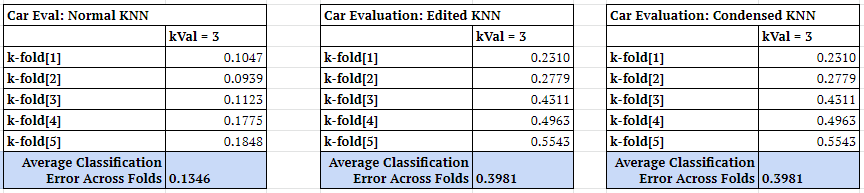
\includegraphics[scale=.7]{CV_ALL_Results}\newline
\end{table}

\begin{table}[h]
		\centering
		\caption{Breast Cancer: ID3 - Experimental Results}
		\label{tab:table2}
		%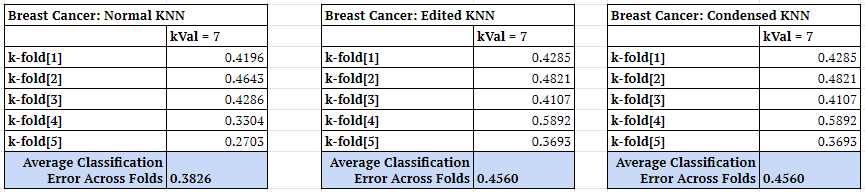
\includegraphics[scale=.7]{BC_ALL_Results}\newline
\end{table}

\begin{table}[h]
		\centering
		\caption{Congressional Vote: ID3 - Experimental Results}
		\label{tab:table3}
		%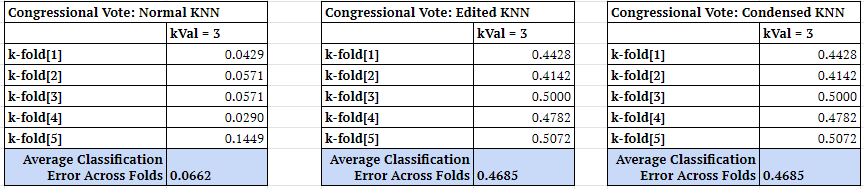
\includegraphics[scale=.7]{CVote_ALL_Results}\newline
\end{table}

\begin{table}[h]
	\centering
	\caption{Albalone: CART - Experimental Results}
	\label{tab:table4}
	%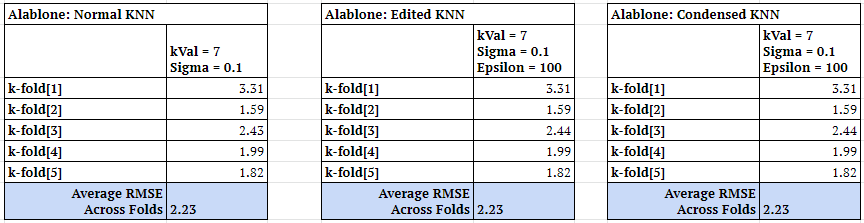
\includegraphics[scale=.7]{ABL_ALL_Results}\newline
\end{table}

\begin{table}[h]
	\centering
	\caption{Computer Hardware: CART - Experimental Results}
	\label{tab:tale5}
	%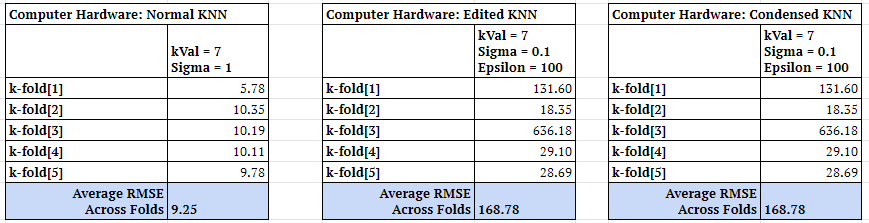
\includegraphics[scale=.7]{CH_ALL_Results}\newline
\end{table}

\begin{table}[h]
	\centering
	\caption{Forest Fires: CART - Experimental Results}
	\label{tab:table6}
	%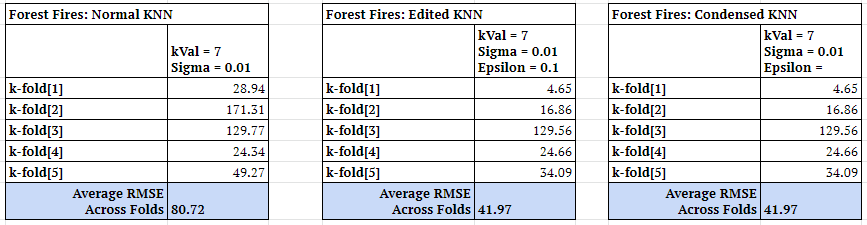
\includegraphics[scale=.7]{FF_ALL_Results}\newline
\end{table}



\newpage

\section{Discussion}
\hspace*{10mm} 

\section{Conclusion}
\hspace*{10mm} 

\section{References}
1. Alpaydin, E. (2004). Introduction to machine learning (Oip). Mit Press. 

\newpage


\end{document}